\begin{slikaDesno}{fig/L_proxy.pdf}
\PID 
Прецизан сензор отклона може се конструисати помоћу процепа у магнетском колу. На слици је приказано
танко торусно језгро, укупне дужине средње линије $\ell = \ell_1 + \ell_2 = 50\unit{cm}$, униформне површине 
попречног пресека $S = 4\unit{cm^2}$ које је по једној 
равни пресечено на два дела. Торус је од магнетски меког гвожђа, велике релативне магнетске пермеабилности 
$\upmu_{\rm r} = 100$. На један део је равномерно и густо намотано $N = 100$ завојака танке бакарне жице. 
Процеп између делова торуса $d$ може да се мења, и представља величину коју овај сензор мери. 
\end{slikaDesno}
 
\begin{enumerate}[label=(\alph*)]
\item У завистности од процепа $d \ll \ell$, изразити индуктивност која се види на прикључцима намотаног калема, $L = L(d)$. 
    Магнетско расипање занемарити.
\item Скицирати зависност индуктивности од ширине процепа у интервалу вредности $100\unit{\upmu m} < d < 3\unit{mm}$
\end{enumerate}

\RESENJE 

Магнетско коло описано је Амперовим законом које се расписује за средњу линију у облику 
$\oint_C {\bf H}\, \de{\bf l} = I_{\rm kroz, C}$. Записивањем тог резултата за средњу линију торуса има се 
\begin{equation}
H_{\rm j} \underbrace{(\ell - 2d)}_{\approx \ell} + H_{\rm p} \cdot 2 d = N I, \label{eq:\ID:amper}
\end{equation}
где су 
$H_{\rm j}$ и $H_{\rm p}$ јачина магнетског поља у језгру и у процепу респективно, а $I$ је јачина струје која 
се успоставља у намотају. Сматрајући да нема 
магнетског расипања, због униформног попречног пресека система, магнетска индукција у систему је константна 
и износи $B = \upmu_0 H_{\rm p} = \upmu_0 \upmu_{\rm r} H_{\rm j}$, па се заменом у \ref{eq:\ID:amper} добија интензитет магнетске 
индукције   
\begin{equation}
    \dfrac{\ell}{\upmu_0 \upmu_{\rm r} } B + \dfrac{2d}{\upmu_0} B = NI
    \Rightarrow
    B = \dfrac{\upmu_0 \upmu_{\rm r} NI}{{\ell} + {2\upmu_{\rm r} d}  }
    \label{eq:\ID:Brez}
\end{equation}
Магнетски флукс који онда постоји у језгру је $\Upphi_{\rm j} = BS$, а укупан магентски флукс намотаја је 
флукс језгра који продире свих $N$ завојака, односно $\Upphi = N\Upphi_{\rm j} = NBS$. Заменом резултата из 
\ref{eq:\ID:Brez} се добија израз за индуктивност која се види на прикључцима намотаја
\begin{equation}
    \Upphi = \underbrace{\dfrac{\upmu_0 \upmu_{\rm r} N^2 S}{{\ell} + {2\upmu_{\rm r} d}  }}_{L} I
\end{equation}

(б) Тражени график у задатом опсегу вредности је дат на слици \ref{fig:\ID:graf}. 

\begin{figure}[ht!]
    \centering
    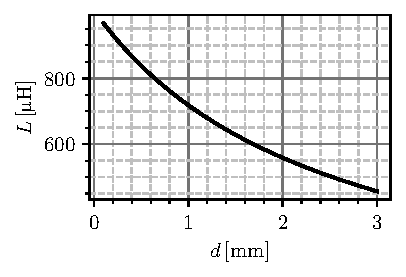
\includegraphics[scale=1]{fig/L_rez.pdf}
    \caption{Уз решење.}
    \label{fig:\ID:graf}
\end{figure}
Приметимо на основу резултата \ref{eq:\ID:Brez}, да је процеп $d$ увећан за $\upmu_{\rm r}$ пута, што је велики број. На тај начин, 
са добрим магнетским материјалом се поље усмерава да прати језгро док практично магнетски отпор пружа само сам процеп. То 
је основни разлог за велику резолуцију мерног инструмента који је базиран на овом принципу.